\documentclass[9pt]{extarticle}
\usepackage{amsmath}
\usepackage{bm}
\usepackage{graphicx}
\usepackage[utf8]{inputenc}
\usepackage{caption}
\usepackage{subcaption}
\title{Finite Element Method}
\author{Student \# }

\begin{document}
\maketitle

\section{Introduction}



The linear elasticity equation

\begin{equation}
\label{eq:linEl}
\nabla \bm{\sigma}(\bm{u}) = - \bm{f}.
\end{equation}

describes deformation and motion on a solid object. In this report, we will present how the linear elasticity equation is applied to a geometry in 3D using the finite element method. We will look at the convergence rate on our methods, and visualize how a bridge is deformed when a car drives over it. We will also look at stress on the bridge and explain parts of our algorithm.



\section{Presentation of the 2D system}

First, let us present some basic results in 2D. Using the finite element method we have made a 2D solver for the linear elasticity problem on a domain $\Omega$. The domain is divided into triangles, called elements, each with 3 nodes. Each node represents an entry in the displacement vector

\begin{equation}
\bm{u}(x,y) = 
\begin{bmatrix}
u_x \\
u_y
\end{bmatrix},
\end{equation}
which is a measure of how much each spatial point has moved. The strain $\bm{\epsilon}$ measures how much each spatial point has deformed and the stress $\bm{\sigma}$ measures how much forces per area are acting on a spatial point. The relations between the displacement, strain and stress are listed in \cite{note2}, and we will go thoroughly through this for the 3D case. Before doing that, let us show that our 2D solver is correct by looking at the error when increasing the grid size.





% 2D problem:



\subsection{Convergence analysis}

We test our code on the problem 

\begin{align}
f_x = \frac{E}{1-\nu^2} (-2y^2 - x^2 + \nu x^2 - 2\nu xy -2xy + 3 - \nu) \\
f_y = \frac{E}{1-\nu^2} (-2x^2 - y^2 + \nu y^2 - 2\nu xy -2xy + 3 - \nu) 
\end{align}

with homogeneous Dirichlet boundary conditions on all boundaries. Compared to the analytical solution 

\begin{align}
\bm{u}(x,y) = \begin{bmatrix}
\, (x^2-1)(y^2-1) \, \\
(x^2-1)(y^2-1)
\end{bmatrix}
\end{align}

we get the error plot shown in Figure \ref{error}. Also, increasing the grid size in each spatial direction by a factor 2, we obtain an accuracy convergence of order 2, as shown in Figure \ref{convergence}. This implies that our code is correct.

\begin{figure}
\center
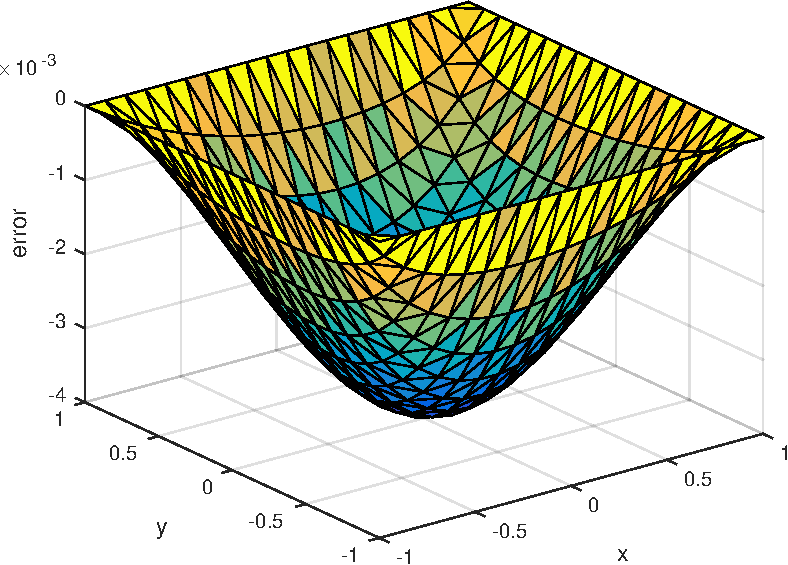
\includegraphics[width=0.4\textwidth]{error_linEl}
\caption{Error between the numerical solution to the linear elasticity problem and the analytical solution with $N = 20$ grid points in each spatial direction. The numerical solution is smaller than the analytical solution.}
\label{error}
\end{figure}

\begin{figure}[ht]
\center
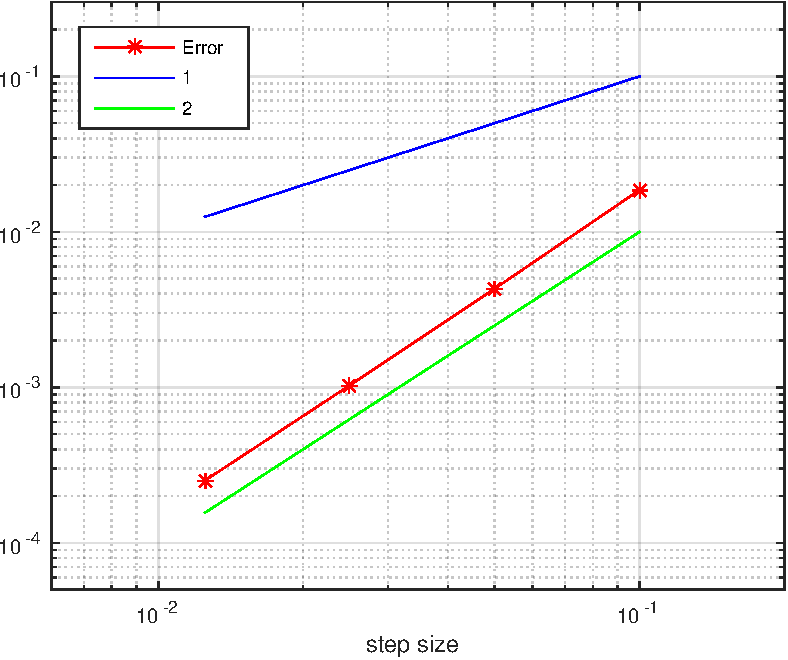
\includegraphics[width=0.4\textwidth]{conv_linEl}
\caption{Loglog plot of the error showing convergence of order 2 of the linear elasticity problem with $N =$ 10, 20, 40 and 80 grid points in each spatial direction. }
\label{convergence}
\end{figure}





% 3D problem:
\section{Presentation of the 3D system}
Modifying the solver to 3D, we get the same relations as in 2D  \cite{note2}. The relation between stress and strain over one element is

\begin{equation}
\label{stress-strain}
\bm{\sigma}^e = \bm{C} \, \bm{\epsilon}^e,
\end{equation}
where
\begin{align*}
\bm{\sigma}^e =
\begin{bmatrix}
\sigma_{xx} \\
\sigma_{yy} \\
\sigma_{zz} \\
\sigma_{xy} \\
\sigma_{yz} \\
\sigma_{xz}
\end{bmatrix}, \,
\bm{\epsilon}^e = 
\begin{bmatrix}
\epsilon_{xx} \\
\epsilon_{yy} \\
\epsilon_{zz} \\
\epsilon_{xy} \\
\epsilon_{yz} \\
\epsilon_{xz} \\
\end{bmatrix}
\end{align*}
and the stress-strain matrix \cite{stressMatrix}
\begin{align*}
\bm{C} = \frac{E}{(1+\nu)(1-2\nu)}
\begin{bmatrix}
(1-\nu) & \nu & \nu & 0 & 0 & 0 \\
\nu & (1-\nu) & 0 & 0 & 0 & 0 \\
\nu & \nu & (1-\nu) & 0 & 0 & 0 \\
0 & 0 & 0 & \frac{1-2\nu}{2} & 0 & 0 \\
0 & 0 & 0 & 0 & \frac{1-2\nu}{2} & 0 \\
0 & 0 & 0 & 0 & 0 & \frac{1-2\nu}{2}
\end{bmatrix}.
\end{align*}
$E$ is the Young's modulus which is a measure of stiffness, and $\nu$ is the Poisson's ratio describing the ratio between the compression and expansion of a material. Further the relation between strain and displacement over one element is
\begin{align}
\label{strain-displacement}
\bm{\epsilon}^e = \bm{B} \bm{u}^e
\end{align}
where $\bm{u}^e$ is the displacement field over one element with four nodes, each with three spatial displacement directions and $\bm{B}$ is the strain-displacement matrix.
\begin{align*}
\bm{u}^e = 
\begin{bmatrix}
u_{1x} \\
u_{1y} \\
u_{1z} \\
\vdots \\
u_{4z}
\end{bmatrix}, \,
&\bm{B} = 
\begin{bmatrix} \\
\bar{\bm{\partial}} \bm{\phi_1} & \bar{\bm{\partial}} \bm{\phi_2} & \bar{\bm{\partial}} \bm{\phi_3} & \bar{\bm{\partial}} \bm{\phi_4} \\[1em]
\end{bmatrix} \textrm{ and } 
\bar{\bm{\partial}} = 
\begin{bmatrix}
\frac{\partial}{\partial x} & 0 & 0 \\[0.3em]
0 & \frac{\partial}{\partial y} & 0 \\[0.3em]
0 & 0 & \frac{\partial}{\partial z} \\[0.3em]
\frac{\partial}{\partial y} & \frac{\partial}{\partial x} & 0 \\[0.3em]
\frac{\partial}{\partial z} & 0 & \frac{\partial}{\partial x}\\[0.3em]
0 & \frac{\partial}{\partial z} & \frac{\partial}{\partial y} \\
\end{bmatrix}
\end{align*}
with 

\begin{align*}
\bm{\phi_i} = 
\begin{bmatrix}
\phi_{i_x} \\
\phi_{i_y} \\
\phi_{i_z} \\
\end{bmatrix}
\end{align*}

being the $i^{th}$ shape function on the current element. The shape functions are in our case linear, and $\bm{\phi_i}$ must be 1 at the $i^{th}$ node and 0 at the three other nodes. Combining \eqref{stress-strain} and \eqref{strain-displacement}, we end up with the relation between displacement and stress,
\begin{align}
\label{stress-displacement}
\bm{\sigma}^e = \bm{C} \bm{B} \bm{u}^e.
\end{align}
This relation is later used when we know the displacement vector $\bm{u}^e$ from the solution of \eqref{eq:linEl} and want to look at the stress on each node. 











\section{The Finite Element Method in 3D}
\label{sec:FEM}

The linear elasticity equation \eqref{eq:linEl} can be written in matrix form as

\begin{align*}
\begin{bmatrix}
\frac{\partial}{\partial x}, & \frac{\partial}{\partial y}, & \frac{\partial}{\partial z}
\end{bmatrix}
\begin{bmatrix}
\sigma_{xx} & \sigma_{xy} & \sigma_{xz} \\
\sigma_{xy} & \sigma_{yy} & \sigma_{yz} \\
\sigma_{xz} & \sigma_{yz} & \sigma_{zz}
\end{bmatrix} = -
\begin{bmatrix}
f_x, & f_y, & f_z 
\end{bmatrix}.
\end{align*}

Let us for simplicity assume homogeneous Dirichlet boundary conditions on $\partial \Omega_D$. Multiplying with a test function $\bm{v}$ and integrating over the domain $\Omega$, we end up with the weak formulation. 

\begin{equation}
\int_\Omega \bm{\epsilon}(\bm{v})^T \bm{C} \bm{\epsilon}(\bm{u}) \, d\Omega = \int_\Omega \bm{v}^T \bm{f} \, d\Omega
\end{equation}

Now, we substitute the test function by linear basis functions $\bm{v} = \bm{\phi_i}$ and skipping some details we end up with the linear system for one element,

\begin{equation}
\label{eq:linear-system}
\bm{A}^e \bm{u}^e = \bm{b}^e.
\end{equation}

$\bm{A}^e$ is the stiffness element matrix,

\begin{align}
\bm{A}^e = \int_\Omega \bm{B}^T \bm{C} \bm{B} \, d\Omega = \bm{B}^T \bm{C} \bm{B} \cdot V^e
\end{align}
where $V^e$ is the volume of the current element. Because the integrand is constant, we can substitute the integral by the volume of the domain. $\bm{b}^e$ is the element load vector with the $i^{th}$ element 

\begin{align}
\label{eq:load-vector}
b^e_i = 
\int_{\Omega} \bm{\phi_i} \bm{f} \, d\Omega.
\end{align}

If $\bm{f}$ is a constant in the element (typically a result of mass density) then \eqref{eq:load-vector} can be calculated exact by a 1 order Gauss quadrature, since the basis functions are linear. 

We have now presented a linear system for one element. Iterating over all elements, and mapping to a stiffness matrix $\bm{A}$ and load vector $\bm{b}$, we obtain a linear system for all the nodes in our geometry. 

\begin{equation}
\bm{A} \bm{u} = \bm{b}
\end{equation}

with $\bm{u}$ being the displacement vector for all the nodes in the system. The load vector $\bm{b}$ is a $3n$-vector with 3 spatial directions in each node.



\subsection{Convergence analysis in 3D}

Inspired by the convergence test in 2D we test our code on the problem 

\begin{align}
f_x = &K^* \left[-2(y^2-1)(z^2-1) + (2 \nu -1)(x^2-1)(z^2 +y^2-2) \right.\nonumber\\
 &\left. -2x(y(z^2-1) + z(y^2-1)) \right] \\
 f_y = &K^* \left[-2(x^2-1)(z^2-1) + (2 \nu -1)(y^2-1)(z^2 +x^2-2) \right.\nonumber\\
 &\left. -2y(x(z^2-1) + z(x^2-1)) \right] \\
 f_z = &K^* \left[-2(x^2-1)(y^2-1) + (2 \nu -1)(z^2-1)(y^2 +x^2-2) \right.\nonumber\\
 &\left. -2z(x(y^2-1) + y(x^2-1)) \right] \\
 K^* = & \frac{E \nu}{(1+\nu)(1-2\nu)},
\end{align}
on the reference cube $(-1,1)^3$ with homogeneous Dirichlet boundary conditions on all boundaries. This problem has the analytical solution

\begin{align}
\bm{u} = \begin{bmatrix}
\, (x^2-1)(y^2-1)(z^2-1) \, \\
\, (x^2-1)(y^2-1)(z^2-1) \, \\
(x^2-1)(y^2-1)(z^2-1)
\end{bmatrix}.
\end{align}
As can be seen in figure \ref{fig:convergence3d} we have linear convergence in 3d.

\begin{figure}
\center
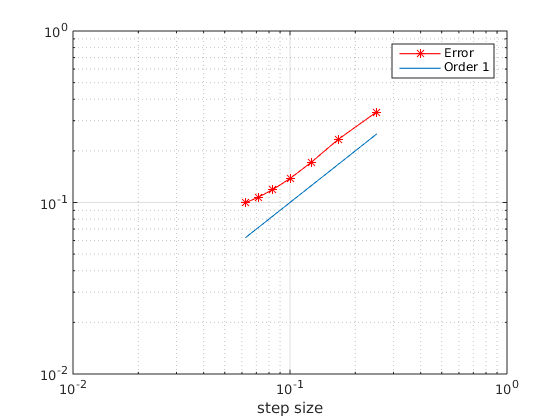
\includegraphics[width=0.4\textwidth]{convergence3d}
\caption{Logarithm error convergence plot for the 3d case, with N = 4, 6, 8, 10, 12, 14, 16 grid points in each spatial direction.}
\label{fig:convergence3d}
\end{figure}



%Stress analysis
\section{Stress analysis}

The code has so far only calculated the displacement in the geometry. The stress $\bm{\sigma}$, which measures how much forces per area are acting on a particular spatial point, is very interesting when it comes to how much an object can withstand. To do a stress analysis we loop over all elements and using the relation \eqref{stress-displacement} we get the element stress vector for each element.

Of special interest is the Von Mises stress \cite{VonMises}, a scalar representation of the stress, since this can be directly compared to the materials yield strength to look for permanent displacement. The Von Mises stress is calculated as 

\begin{align*}
\sigma_{v} = \sqrt{ \frac{1}{2} \left[  (\sigma_{xx} -\sigma_{yy})^2 + (\sigma_{yy} -\sigma_{zz})^2 + (\sigma_{zz} -\sigma_{xx})^2 + 6\left(\sigma_{xy}^2 + \sigma_{yz}^2 + \sigma_{xz}^2 \right) \right]}.
\end{align*}


The Von Mises stress is saved for every element, and to get the nodal stress we average the neighboring elements. If the nodal stresses are larger then the material yield strength, we'll get a permanent deformation.


%Our geometry (bridge)
%Figures

\section{Bridge}

\begin{figure}
\center
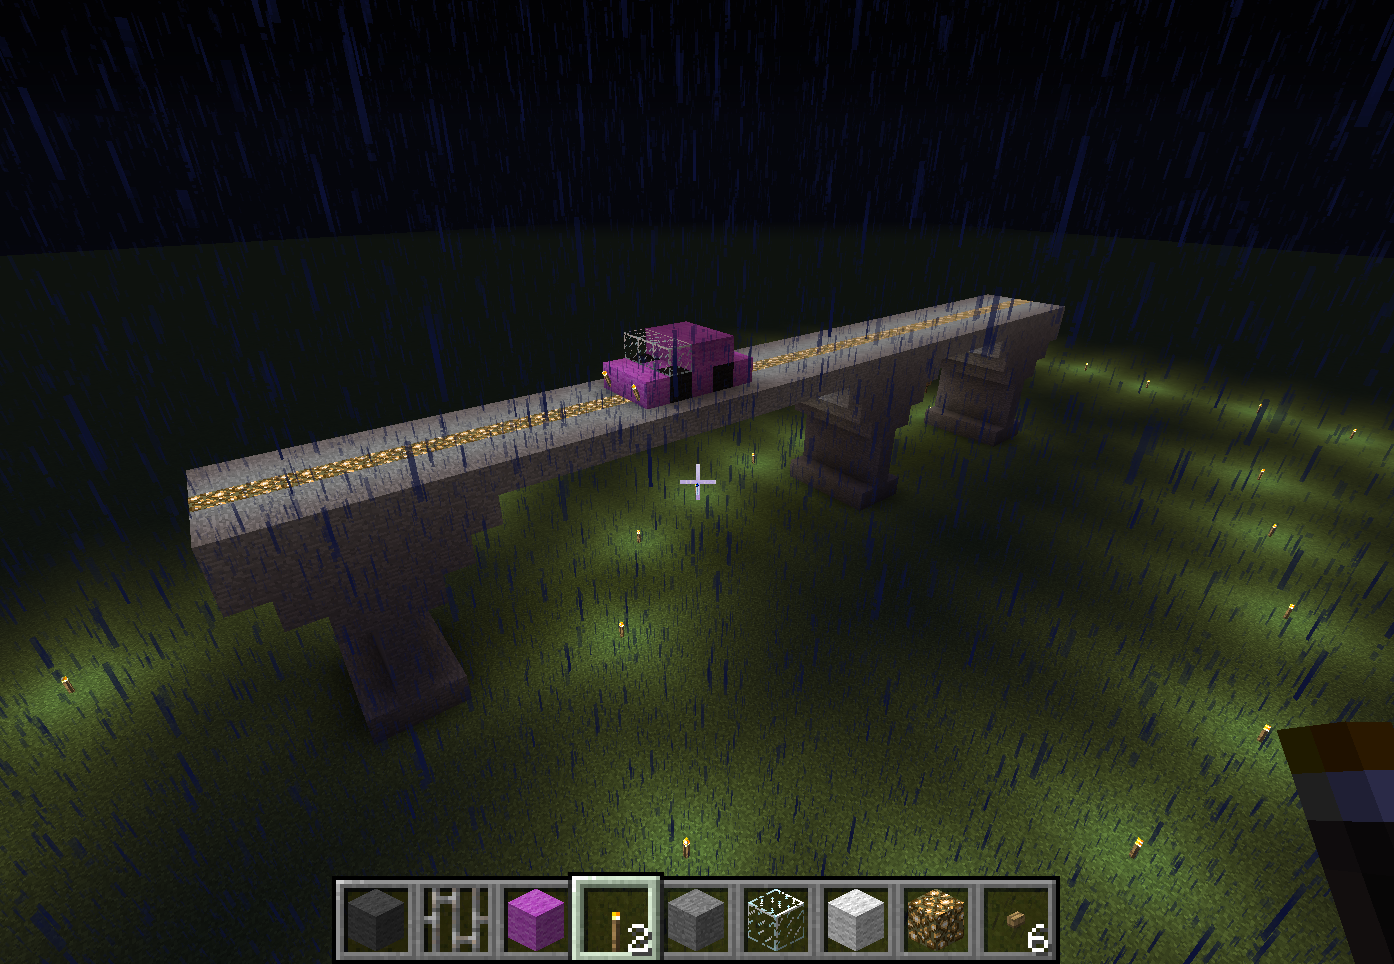
\includegraphics[trim=0cm 5cm 7cm 7cm, clip=true, width=0.9\textwidth]{pic_bridge}
\caption{A picture of the bridge we built in minecraft.}
\label{fig:picBridge}
\end{figure}


For this section we ventured ahead and built ourselves a bridge in minecraft as shown in Figure \ref{fig:picBridge}. Importing the bridge into matlab was, apart from some tedious work, quite straight forward.


\subsection{Short overview of algorithm}
Since we wanted to have some kind of time-dependency on our chosen problem, we incorporated a car driving over the bridge. This required us to manually link together the meshes for the bridge and car, and is done in the \textit{mergeBridgeCar.m} matlab function. The supplied \textit{hex2tetr.m} function is used to split our minecraft cubes into fitting tetrahedrons. We find the boundary points at $z = 0$, and pass the whole thing into \textit{FEM.m} which solves the linear elasticity problem using the finite element method further specified in Section \ref{sec:FEM}. The function \textit{stressRecovery.m} recovers the nodal Von Mises stresses by averaging the element neighbor stresses for each node. The stress is found by REF.


\subsection{Materials chosen}
\begin{table}
\center
\caption{Material constants for oak wood used in the bridge.} 
\begin{tabular}{cc}
Material constant & Value \\ 
\hline 
Young's modulus & 11 GPa \\ 
Density & 650 kg/m$^3$ \\ 
Compressive yield strength & 46 MPa \\ 
Poissons ratio & 0.3 \\ 
\label{tab:oak}
\end{tabular}
\end{table}


For this problem we chose the material of the bridge to be oak wood. We defined the dimension of one minecraft block to be a cubic meter. The material constants we needed for wood were the averaged values we found at \cite{oak} and the value for the Poisson's ratio was conveniently set to 0.3. All the material constants are presented in table \ref{tab:oak}. We really wanted to see what happens when a heavy car drives over the bridge, so we defined the car to be extremely heavy. The result of this is visualized in Figure \ref{fig:bridget8t23}.




\begin{figure}[ht]
        \centering
        \begin{subfigure}[b]{0.45 \textwidth}
                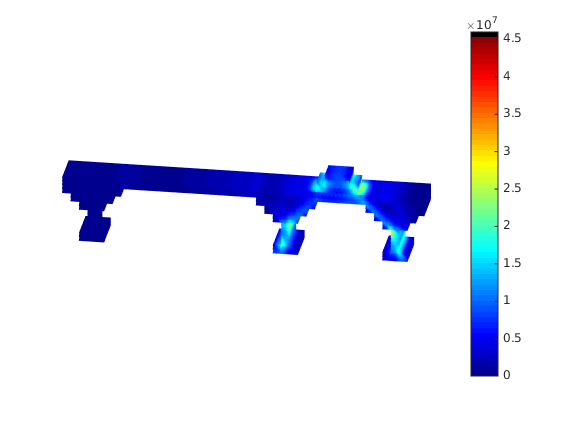
\includegraphics[width=\textwidth]{time080}
                \caption{The car after 8 seconds have passed.}
        \end{subfigure}
        ~
        \begin{subfigure}[b]{0.45 \textwidth}
                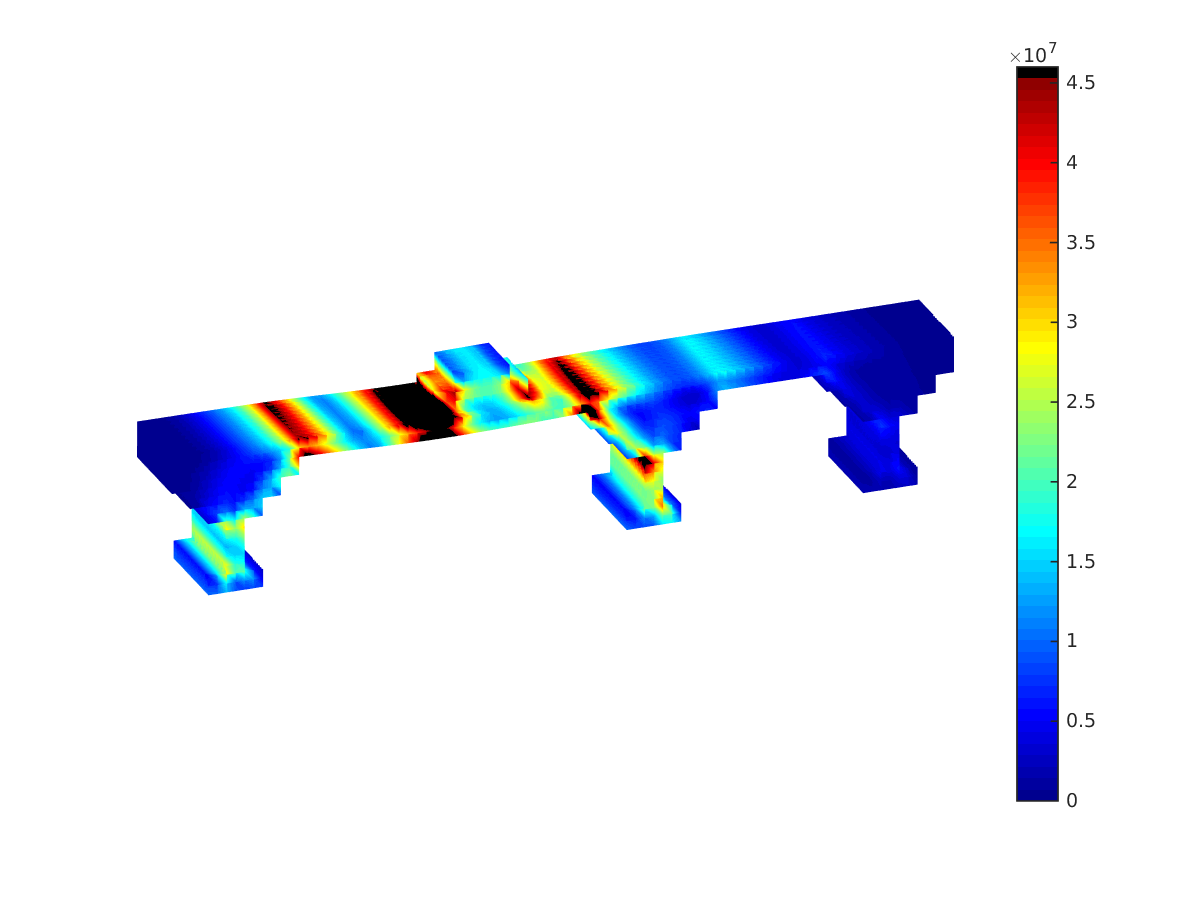
\includegraphics[width=\textwidth]{time230}
                \caption{The car after 28 seconds have passed.}
        \end{subfigure}
        \caption{The (really) heavy car driving over the bridge at 1 m/s. The Von Mises stress is plotted as the varying color. If the Von Mises stress is higher than the material yield, it is painted black (and the bridge will be permanently deformed). We see that at time = 28 the bridge has been severely damaged. }
        \label{fig:bridget8t23}
\end{figure}



%Problems along the way
\section{Challenges}

Throughout the process, we did face some challenge. We will not present all to you, but some of the most important ones. 

When making the load vector in 3 dimensions, we forgot to map load vector to the right nodes. This resulted in weird displacements, see Figure REF. 








%Conclusion, discussion



\begin{thebibliography}{3}

\bibitem{stressMatrix}
	Colorado University\\
	\emph{http://www.colorado.edu/engineering/cas/courses.d/IFEM.d/IFEM.Ch14.d/\\IFEM.Ch14.pdf}


\bibitem{stressRecovery}
	Colorado University\\
	\emph{http://www.colorado.edu/engineering/cas/courses.d/IFEM.d/IFEM.Ch28.d/\\IFEM.Ch28.pdf}	



\bibitem{stress}
Wikipedia - Stress (mechanics) \\
\emph{http://en.wikipedia.org/wiki/Stress\_ (mechanics)}

\bibitem{VonMises}
Wikipedia article on Von Mises Stress \\
\emph{http://en.wikipedia.org/wiki/Von\_Mises\_yield\_criterion}

\bibitem{note2}
Some rought theoretical background for the programming project in TMA4220 - part 2 \\
Kjetil André Johannesen \\
\emph{Bake, shake or break - and other applications for the FEM}

\bibitem{oak}
	Wolfram alpha entry for "oak wood"\\
	\emph{http://www.wolframalpha.com/input/?i=oak+wood}
	



\end{thebibliography}




\end{document}
